\documentclass[a4paper]{siamart190516}

\usepackage{damacros}

% Sets running headers as well as PDF title and authors
\headers{Preliminary notes}{Daniele, Sage, and Zack}

% Title. If the supplement option is on, then "Supplementary Material"
% is automatically inserted before the title.
\title{Notes on RBFs methods for Neural Fields} 

% Authors: full names plus addresses.
\author{%
  Daniele 
  \and
  Sage 
  \and 
  Zack 
  % \thanks{%
  %   Vrije Universiteit Amsterdam,
  %   Department of Mathematics,
  %   Faculteit der Exacte Wetenschappen,
  %   De Boelelaan 1081a,
  %   1081 HV Amsterdam, The Netherlands.
  % \protect\\
  %   Inria Sophia Antipolis M\'editerran\'ee Research Centre,
  %   MathNeuro Team,
  %   2004 route des Lucioles-Boîte Postale 93 06902,
  %   Sophia Antipolis, Cedex, France.
  % \protect\\
  %   (\email{d.avitabile@vu.nl}, \url{writemywebpage}).
  % }
  % % \and
% %   Paul T. Frank \thanks{Department of Applied Mathematics, Fictional University, Boise, ID 
% % (\email{ptfrank@fictional.edu}, \email{jesmith@fictional.edu}).}
% % \and Jane E. Smith\footnotemark[3]
}

\graphicspath{{./Figures/}}

\begin{document}

\maketitle

\begin{abstract}
  Preliminary notes on RBFs for neural fields
\end{abstract}
  
\section{Example of collocation scheme for a neural field on a ring} 
Let us consider a neural field model on a ring, with cosine synaptic kernel, 
\begin{equation}\label{eq:NFRing}
  \begin{aligned}
 & \partial_t u(x,t) =  -u(x,t) + g(x,t)+ \int_{-\pi}^{\pi} \cos(|x-y|) f(u(y,t)) dy,
   \qquad x \in [-\pi,\pi) \\
 & u(x,0) = v(x) 
  \end{aligned}
\end{equation}
where $g$, $f$, and $v$ are prescribed functions, and let us derive an intuitive scheme
for this problem. We pick $n+1$ evenly spaced points in $[-\pi,\pi]$
\begin{equation}\label{eq:nodesRing}
  x_i = -\pi + h i, \qquad h = \frac{2\pi}{n}, \qquad i = 0, \ldots, n.
\end{equation}
Because of periodicity, we expect to need only $n$ of those $n+1$ points, and indeed
this turns out to be the case. If $v(x)$ is a periodic function, applying the
trapezium rule with the grid above gives (note the sum runs over just $n$ points)
\[
  \int_{-\pi}^{\pi} v(y)\,d y \approx \sum_{j=1}^{n} v(x_j) h.
\]
The integrand in \cref{eq:NFRing} is periodic in $y$, so we evaluate the neural
field at $x_1, \ldots, x_n$ ($x_0$ excluded) and simultaneously apply the quadrature rule
above to obtain
\[
  \begin{aligned}
  & U'_i(t) = -U_i(t) + \sum_{j=1}^{n} \cos(x_i - x_j) f(U_j(t)) h + G_i(t), \qquad i = 1,\ldots,n  \\
  & U_i(0) = V_i
  \end{aligned}
\]
that is, a system in the form 
\begin{equation}
  \begin{aligned}
   &  U'(t) = - U(t) + M F(U(t)) +  G(t)\\ 
   &  U(0) = V
  \end{aligned}
\end{equation}  
in which $U(t), G(t), F(U(t)), V$ are vectors in $\RSet^n$ for all $t$, and in which
$M$ is the $n$-by-$n$, full matrix entries $M_{ij} = \cos(x_i - x_j)h$. The intention
here is to use $U_i(t)$ as an approximation for $u(x_i,t)$.

The scheme above is an example of \textit{collocation scheme}. Even though this may
not be apparent from the quick presentation above, it scaffolding is polynomial
approximation, and more specifically polynomial interpolation. If we
look at the scheme with the right lenses, we find that many important properties of
the scheme revolve around solving following problem: 
\begin{problem}[Interpolation problem]\label{prob:interpolation}
Given a function $v(x)$, and a set of $n$ points $\{ x_i \}_{i=1}^n$, find a function
$v_n(x)$ such that 
\[
  v(x_i) = v_n(x_i), \qquad i = 1,\ldots, n.
\]  
Once $v_n$ is constructed, study how well $v_n(x)$ approximates $v(x)$ away from the
nodes $x_i$, for instance by studying $\| v - v_n \|$ as $n \to \infty$ in a suitable
norm.
\end{problem}
The problem above is cast in terms of a generic function $v(x)$, but thinking of this
function $v$ as being the initial condition of the neural field \cref{eq:NF} is
useful.

In \cite{Avitabile:2023ab} it is shown that the scheme discussed
above stems from the following choices: 
\begin{enumerate}
  \item The points are evenly spaced in $[-\pi,\pi]$.
  \item The function $v_n$ that subtends the scheme is of the following form:
    \begin{equation}\label{eq:LagrangeInterp}
      v_n(x) = \sum_{j=1}^{n} v(x_j) \ell_j(x), 
    \end{equation}
    where $\ell_i(x)$ are Lagrange polynomials, hence $\ell_i(x_j) = \delta_{ij}$.
    This choice of $v_n$ is one way to solve the interpolation
    \cref{prob:interpolation}.
\end{enumerate}
In \cite{Avitabile:2023ab} it is also shown that a variety of
other schemes, of Finite Elements or Galerkin type, are analysable following a common
framework.

\subsection{RBFs for Neural field equations}\label{ssec:RBFMotivation} From a
numerical standpoint, the discussion above brings about the following questions:
  \begin{itemize}
    \item How to choose a parsimonious distributions of points? Under which conditions
      is a homogeneous point distribution a good idea? What if we are in multiple
      spatial dimensions? What if the cortex has curvature, as a manifold in 3D? How
      to handle refinements?
    \item The interpolation function $v_n$ given in \cref{eq:LagrangeInterp} is one
      of many possible choices. Can we gain by changing the form of $v_n$, and
      perhaps pairing it to a point distribution that ``goes well with $v_n$"?
    \item Evaluating the right-hand side of system \cref{eq:NFODE} involves a
      matrix-vector multiplication with a dense matrix $M$. This means the scheme
      won't scale well on large cortices, because at each time step it takes
      $O(n^2)$ operations to evaluate the right-hand side. Can we choose points $\{
      x_i \}$, interpolant $v_n$, and quadrature rules so that $M$ is sparse?
  \end{itemize}

  Using RBFs is promising and interesting because of the following points:
  \begin{itemize}
      \item RBF handle point distributions in a flexible and adaptable manner. They
        work well in multiple spatial dimensions, and on curved geometries. It is is
        relatively simple to add points where it is needed; RBFs are constructed
        using translates of a kernel function, without a mesh.
      \item Convergence results for RBFs seem available in literature, so there is
        hope to connect to the framework in
        \cite {Avitabile:2023ab} and quickly obtain convergence
        rates.
      \item We will focus on RBF interpolants of the form
        \begin{equation}\label{eq:RBFInterpolation}
          v_n(x) = \sum_{i=1}^{n} \sum_{j=1}^{k_i} V_{ij} \Phi(\| x - \xi_{ij} \|),
        \end{equation}
        where $\xi_{ij}$ are suitably chosen subsets of $\{ x_i \}$, as we will
        specify later. This form of interpolation induces a \textit{sparsification}
        of the matrix $M$.
  \end{itemize}
    
\subsection{Main objectives of this work}\label{ssec:Objectives} An interesting
self-contained publication could be centred around the following:
\begin{itemize}
  \item Describe collocation schemes for generic neural fields posed on surfaces,
    using RBFs as the underlying interpolants.
  \item If at all possible, infer the convergence rate of these schemes. If not,
    present an empirical convergence scheme on a simple model such as
    \cref{eq:NFRing} (or perhaps a 2D version of it).
  \item Showcase the method on a realistic cortical geometry, using either a
    multi-layer neural field, or a Montbrio version of neural field.
  \item If we want, give people simple routines to solve neural fields.
\end{itemize}
Possibly in a separate publication, we could look at the problem with diffusion, and
time adaptivity.

\section{Notation}\label{sec:notation} We will use the index sets by $\NSet_n = \{
1,\ldots, n\}$. In addition, we will endow $\RSet^n$ with the standard Euclidean
norm, which we shall denote by $\|\blank\|_2$, or simply $\| \blank \|$.

\section{Heuristic scheme formulation}\label{sec:model} To understand how RBFs enter
into the discretisation, we show how interpolation determines the collocation scheme,
that is, how the choice of $v_n$ translates into a collocation scheme. The purpose of
this section is to prepare us for that: no mention will be made yet about
interpolation, or $v_n$, but we are getting ready for that.

Let us consider a neural field posed on
a compact domain $D \subset \RSet^d$
\begin{equation}\label{eq:NF}
  \begin{aligned}
  &
  \begin{aligned}
    \partial_t u(x,t) =  -u(x,t)  &+ g(x,t) \\
                & + \int_{D} w(x,y) f(u(y,t))d \mu(y),
  \end{aligned}
  && (x,t) \in D \times [0,T] \\
  & u(x,0) = v(x) && x \in D 
  \end{aligned}
\end{equation}
It is assumed here that the integral is on a manifold, hence it is expressed in terms
of a measure $\mu$. Heuristically, a collocation scheme for \cref{eq:NF} can be conceived
in steps, as follows:

\textbf{Step 1: nodes selection.} Pick $n$ points in the domain $D$. We denote them by
$\Xi = \{ x_i \}_{i \in \NSet_n} \subset D$. In what follows, it may be useful to
make $n$ depend on a positive real number $h$, a discretisation parameter, so that
$n(h) \to \infty$ as $h \to 0$, or as $h \to \infty$. An example of such relationship
is given in \cref{eq:nodesRing}. We will omit the dependence of $n$ on $h$ when
possible. 

\textbf{Step 2: Collocation.} 
Impose that \cref{eq:NF} holds at each node (\textit{collocate the equation} at
each $x_i \in \Xi$). This means replacing \cref{eq:NF} by a set of $n$ equations
\begin{equation}\label{eq:NFColl}
  \begin{aligned}
  &
  \begin{aligned}
    \partial_t u_n(x_i,t) =  -u_n(x_i,t) &+ g(x_i,t) \\
                & + \int_{D} w(x_i,y) f(u_n(y,t))d \mu(y),
  \end{aligned}
  && (x_i,t) \in \Xi \times [0,T] \\
  & u_n(x_i,0) = v(x_i) && x_i \in \Xi 
  \end{aligned}
\end{equation}

Comparing \cref{eq:NF} with \cref{eq:NFColl} we note that the latter is expressed in
terms of the unknown $u_n$, which is an approximation to $u$: the two functions
satisfy evolution equations that coincide only at the nodes $\Xi$, not on the whole $D$.
Another observation is that \cref{eq:NFColl} may be useful for theoretical
estimates, but it is clearly not implementable on a computer as is, because integrals must be
approximated. This takes us to the last step.
  
\textbf{Step 3: Quadrature.} Select a quadrature for the integral, and solve
\begin{equation}\label{eq:NFODEQuad}
  \begin{aligned}
   & \tilde \alpha'(t) = -\tilde \alpha(t) + \tilde K(\tilde \alpha(t)) + \gamma(t) \qquad  t \in [0,T],\\ 
   & \tilde \alpha (0) = \nu,
  \end{aligned}
\end{equation}  
where $\tilde \alpha(t)$, $\gamma(t), \tilde K(\tilde \alpha(t)), \nu \in \RSet^n$ with
$\gamma_i(t) = g(x_i,t)$, $\nu_i = v(x_i)$, and where $(\tilde \alpha(t))_i$
approximates $u_n(x_i,t)$. The nonlinear mapping $K(\tilde \alpha)$ involves a matrix-vector
multiplication, and incorporates quadrature weights.

\section{Collocation schemes as interpolatory projection schemes}\label{sec:projectionSchemes} 

Once we have refined the steps of a collocation scheme, we can bring interpolation
into the picture. In \cite{Avitabile:2023ab} it is shown that convergence estimates
for the collocation scheme (and other schemes) are possible disregarding step 3. In
fact, with just steps 1-2 can estimate how fast $u_n$ tends to $u$, as $n \to \infty$.
Once a convergence rate is established, then this instructs which quadrature scheme
to select: the quadrature should respects this rate, so that we can use $(\tilde
\alpha(t))_i$ as an approximation to $u(x_i,t)$, not simply $u_n(x_i,t)$. 

We do not have to get into the details of
\cite{Avitabile:2023ab}, but one aspect is important for these
notes: it is useful to understand how \cref{eq:NFColl} is derived from \cref{eq:NF}
using a projection. The RBFs will provide, in fact, a flexible and accurate
\textit{interpolatory projector}. 

To make progress on this, let us assume we seek for a solution to the neural field
equations in the space of continuous functions $\XSet = C(D)$. A projector $P_n$ is a
linear mapping from $\XSet$ to an $n$-dimensional subspace $\XSet_n \subset \XSet$
such that $P_n (P_n v) = P_n v$ for all $v \in \XSet$. The distinctive feature of an
\textit{interpolatory projector} is that it has the property  
\[
  (P_n v)(x_i) = v(x_i), \qquad x_i \in \Xi,
\] 
that is, $P_n v$ is a function of $x$, which approximates $v(x)$, and it is exact
at the nodes $x_i$. The previous sections contain two interpolatory projectors in
disguise. In \cref{eq:LagrangeInterp} we wrote
\[
  v_n(x) = \sum_{j=1}^{n} v(x_j) \ell_j(x). 
\]
Since $v$ is a continuous function, then so $v \in \XSet$, and $v_n$ is a linear combination
of $\{ \ell_j \}_{j=1}^n$, so $v_n \in \XSet_n = \spn \{ \ell_1, \ldots, \ell_n \}$.
This means we can interpret the previous writing as
\[
  (P_n v)(x) = \sum_{j=1}^{n} v(x_j) \ell_j(x),
\]
that is, $v_n$ is the action of $P_n$ on the function $v$, $v_n = P_n v$.
The same can be said about \cref{eq:RBFInterpolation}, which defines another choice
of the interpolant, and another choice of projector $P_n$. A fundamental property of
interpolatory projectors is the following (see \cite[Proposition
4.1]{Avitabile:2023ab}): \da[]{Cite Atkinson and others} for any
$r \in \XSet$, 
\begin{equation}\label{eq:projCollProperty}
P_n r = 0, 
\qquad \text{if, and only if,} \qquad 
(P_n r)(x_i) = 0, \qquad i \in \NSet_n.
\end{equation}
This property is useful in describing the system in terms of residual, as we shall do
in a moment.

We now revisit the neural field equation and the collocation scheme in terms of the
projector $P_n$. Firstly, we rewrite the neural field equation \cref{eq:NF} in
operator form, as the following Cauchy problem on the Banach space $\XSet$
\begin{equation}\label{eq:cauchy}
  \begin{aligned}
  & U'(t) = - U(t) + WF(U(t)) + G(t) =:  N(t,U(t)), \qquad t \in J, \\
  & U(0) = V.
  \end{aligned}
\end{equation}
The identification with \cref{eq:NF} is established by setting $J = [0,T]$,
$V = v(\blank)$, and
\[  
  \begin{aligned}
   & U \colon J \to \XSet, && t \mapsto u(\blank,t),
   & G \colon J \to \XSet, && t \mapsto g(\blank,t), \\
   & W \colon \XSet \to \XSet, && v \mapsto \int_{D} w(\blank,y) v(y) \,d \mu(y),
   & F \colon \XSet \to \XSet, && v \mapsto f(v). 
  \end{aligned}
\]
Under suitable generic assumptions \da[]{if needed, include them}, the Cauchy problem
is well-posed under general assumptions that is, there is a unique $u \in
C^1(J,\XSet)$ satisfying \cref{eq:cauchy}, see
\cite{Potthast:2009bd,Faugeras:2009gn}, and \cite[Lemma 2.7]{Avitabile:2023ab}.

Secondly, it is possible to interpret \cref{eq:NFColl} in operator form, as
\begin{equation}\label{eq:cauchyPn}
  \begin{aligned}
  & \dot U_n(t) = - U_n(t) + P_n WF(U_n(t)) + P_n G(t) =  P_n N(t,U_n(t)), \qquad t \in J, \\
  & U_n(0) = P_n V,
  \end{aligned}
\end{equation}
which is a Cauchy problem on the space $\XSet_{n}$. This problem is also well-posed
and gives a solution $u_n \in C^1(J,\XSet_n)$ and
\cite[Theorem 3.1]{Avitabile:2023ab}.

Using \cref{eq:projCollProperty}, we can now pass from \cref{eq:cauchyPn} to an
equivalent ODE in $\RSet^n$. We define the residual
\[
  R \colon C^1(J,\XSet) \to C(J,\XSet), \qquad U \mapsto U' - N(\blank, U),
\]
rewrite \cref{eq:cauchyPn} as
\[
  P_n \bigl( R(U_n)(t) \bigr) = 0, \qquad t \in J, \qquad 
  P_n \bigl( U_n(0) - V\bigr) = 0, 
\]
which, by property \cref{eq:projCollProperty} is equivalent to
\[
  \begin{aligned}
  & U'_n(t)(x_i) = \bigl[P_n N(t,U_n(t))\bigr](x_i), \qquad (i,t) \in \NSet_n \times J, \\
  & U_n(0)(x_i) = (P_n V)(x_i).
  \end{aligned}
\]
Finally, since $U_n(t) \in \XSet_n$, we can write $U_n(t) = \sum_{j \in \NSet_n}
\alpha_j(t) \ell_j$ and an ODE on $\RSet^n$,
\begin{equation} \label{eq:NFODE}
  \begin{aligned}
   & \alpha'(t) = -\alpha(t) + K(\alpha(t)) + \gamma(t) \qquad  t \in [0,T],\\ 
   & \alpha (0) = \nu,
  \end{aligned}
\end{equation}  
where 
\[
  \begin{aligned}
  & \alpha_i(t) = U_n(t)(x_i), && \nu_i = v(x_i),  \\
  & \gamma_i(t) = g(x_i,t),
  && K_i(\alpha) = 
    \int_{D}w(x_i,y) f\Bigl( \sum_{j \in \NSet_n} \alpha_j \ell_j(y)\Bigr) \, d\mu(y)
  \end{aligned}
\]
In passing, we note that the system \cref{eq:NFODE} above is related, but not
identical, to \cref{eq:NFODEQuad}. The former is expressed in terms of 
$K \colon \RSet^n \to \RSet^n$, the latter in terms of
$\tilde K \colon \RSet^n \to \RSet^n$, which adopts a quadrature rule to approximate
the integrals in $K$. In the next section, we will give a concrete example of $\tilde
K$

\section{RBF scheme for neural field equations}\label{sec:RBFScheme} 
\begin{figure}
  \centering
  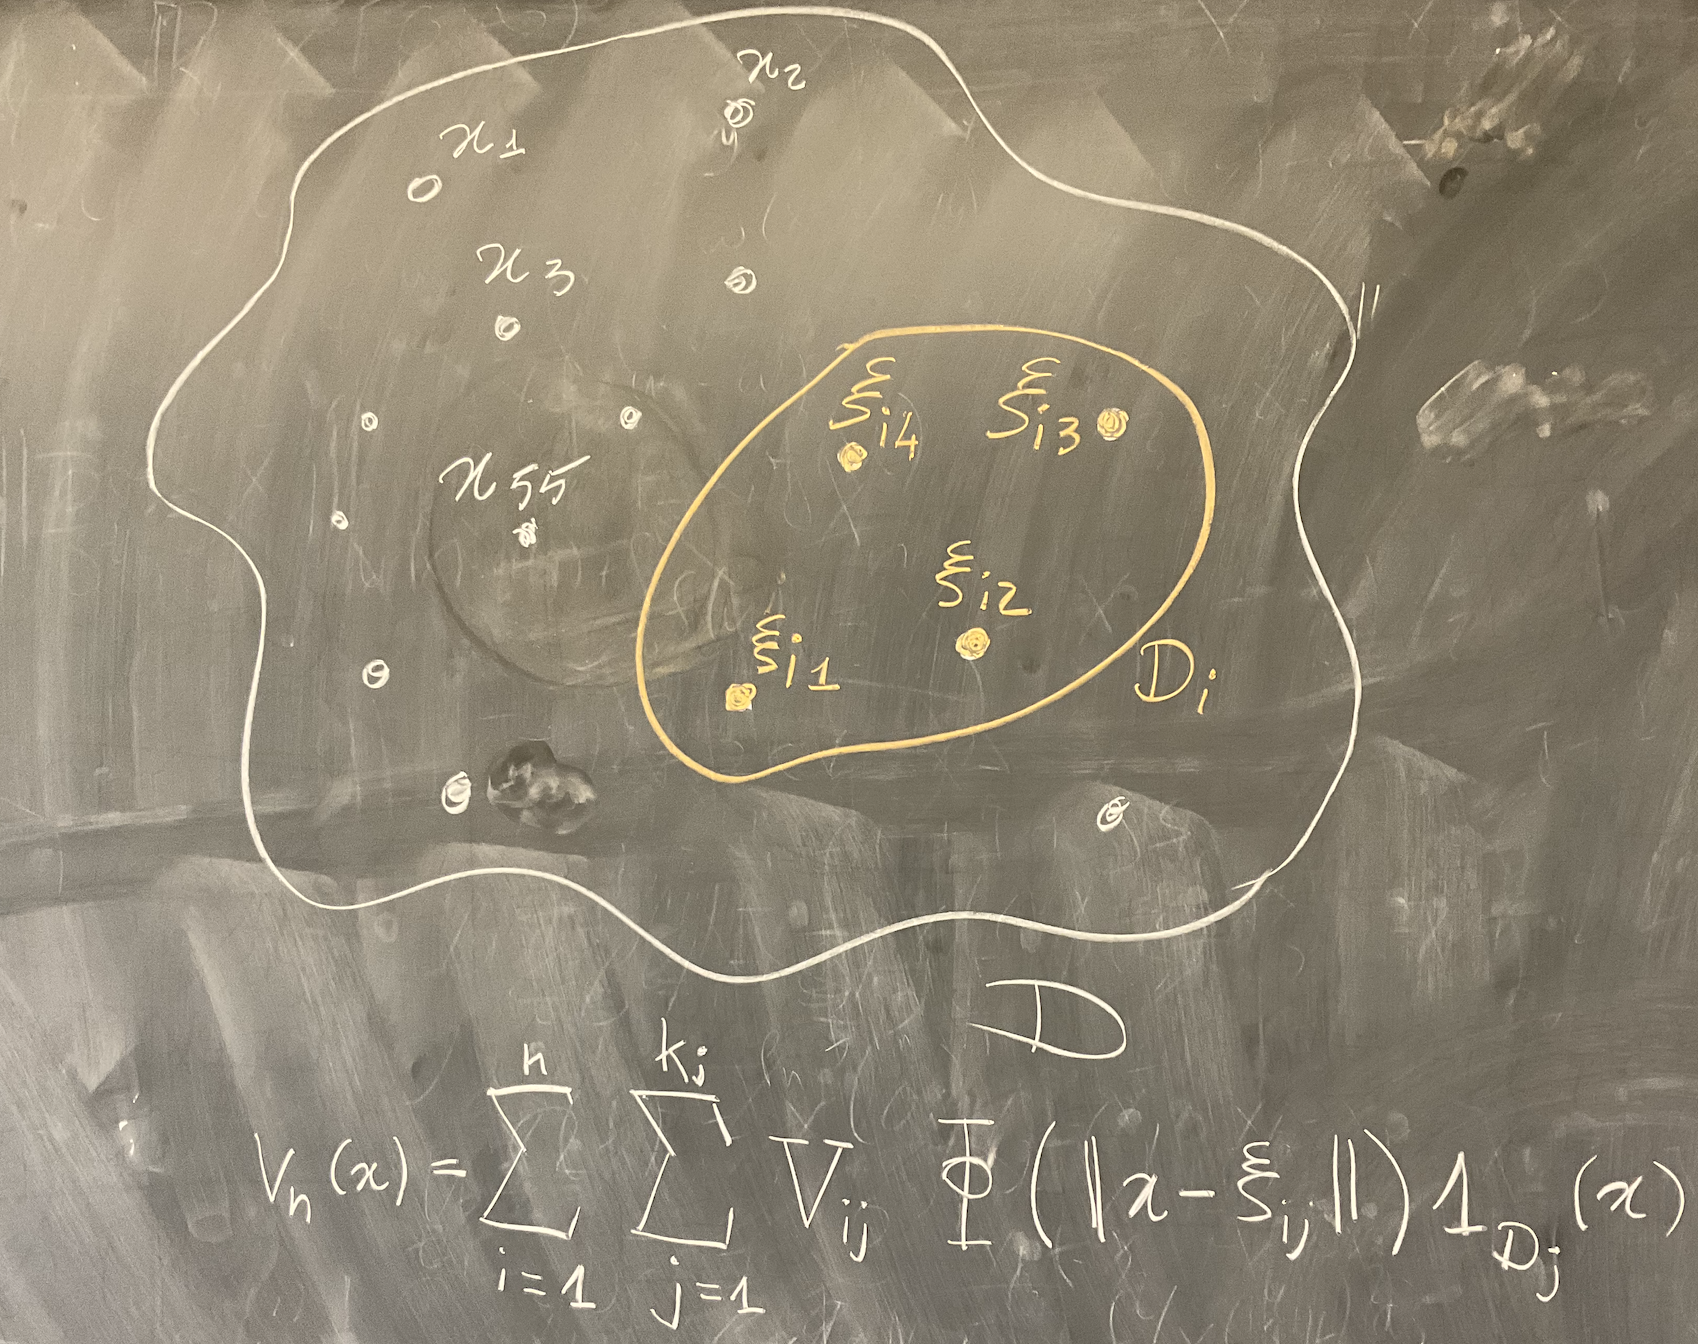
\includegraphics[width=\textwidth]{sketch}
  \caption{The patch $D_i$ of the spatial domain $D$ contains $k_i =4$}
  \label{fig:sketch}
  \da[inline]{We need a meaningful sketch here}
\end{figure}

We now introduce the interpolant we will use in the paper. To define the interpolant
we start from the set of $n$ nodes $\Xi = \{ x_i \}_{i \in \NSet_n}$, with the
associated \textit{Voronoi diagram} $\{ D_i \}_{i \in \NSet_n}$, that is, the
partition of $D$ into cells
\[
  D_i = \Bigl\{ x \in D \colon \| x - x_i \| = \min_{j \in \NSet_n} \| x - x_j \| \Bigr\}.
\]
Further, we consider a map associating each node $x_i$ to $k_i$ nodes $\{\xi_{ij}
\}_{j = 1}^{k_i}$ in $\Xi$, the stencil of $x_i$. More formally we define the
mapping
\[
  S \colon \Xi \to 2^{\,\Xi}, \qquad x_i \mapsto \{ \xi_{ij} \}_{j = 1}^{k_i},
\]
where $2^{\,\Xi}$ is the power set $\Xi$, and denote by $S(x_i)$, or simply $S_i$, the
stencil of node $i$. We stipulate that $x_i$ is part of its stencil, $x_i \in
S(x_i)$. Finally, we define a basic radial function $\phi = \Phi( \| \blank \|)
\colon \RSet^d \to \RSet$, and construct an interpolant of $v$ in the
following form
\begin{equation}\label{eq:RBFExpStencil}   
  v_n(x) = \sum_{j = 1}^{n} \sum_{l=1}^{k_j} V_{jl} \Phi(\| x - \xi_{jl} \|) 1_{D_j}(x) 
\end{equation}
where $1_A$ denotes the indicator function of the set $A \subset \RSet^d$. In
\cref{eq:RBFExpStencil}, the interpolant sums over the stencil in each node, and it
is therefore expressed in terms of $k_1 + \dots + k_n \geq n$ coefficients $\{
V_{jl}\}$. Since $v_n$ interpolates $v$ at the nodes $\Xi$, the coefficients
$V_{jl}$ satisfy the $n$ equations
\[
  v(x_j) = \sum_{l=1}^{k_j} V_{jl} \Phi(\| x_j - \xi_{jl} \|), \qquad j \in \NSet_n.
\]
The system above does not uniquely specify the coefficients $V_{jl}$, and so further
constraints are added,
\da[inline]{Complete this after Sage's input}

Crucially, it is possible to pass from the form \cref{eq:RBFExpStencil} of the
interpolant, to the so-called \textit{cardinal form} of the interpolant, that, is a
Lagrange interpolant
\[
  v_n(x) = \sum_{j=1}^{n} v(x_j) \ell_j(x),
\]
using the transformation
\da[inline]{Complete after Sage's input}

Henceforth, we will use the cardinal form for the analysis and the presentation of
our scheme, while we resort to the stencil-based form to carry out concrete
calculations. The cardinal form of the interpolant defines a projector $P_n \colon \XSet \to
\XSet_n = \spn \{ \ell_1, \ldots, \ell_n \}$, and therefore fits into the framework
presented in the past section.

To complete the scheme, we now require a quadrature formula for the integrand. The
formula we employ is a composite formula over the Voronoi diagram
\[
  \begin{aligned}
  Q v := \int_{D} v(y)\,d \mu(y) 
    & = \sum_{j=1}^n \int_{D_j} v(y) \,d \mu(y) \\
    & \approx \sum_{j = 1}^n \int_{D_j} v_n(y) \,d \mu(y)
      \approx \sum_{j = 1}^n v(x_j) \mu_j =: Q_n v,
  \end{aligned}
\]
in which the integral over a cell $D_i$ is approximated using a single node $x_j$,
the centre of the cell, and a single weight $\mu_j$. The weights satisfy \ldots
\da[inline]{Complete. I am unsure there are two approximation symbols above, or just
one. That depends on how weights are calculated. If possible, we should say something
about the expected convergence rate of $|Qv - Q_nv|$.} We are now ready to specify a discrete scheme by applying the quadrature rule $Q_n$
the function $K$ in \cref{eq:NFODE}, recalling that each $D_i$ contains exactly
one node, namely $x_i$, and obtaining the spatially-discrete scheme
\[
  \begin{aligned}
  & \tilde \alpha'(t) = -\tilde \alpha(t) + \gamma(t) 
    + M f(\tilde \alpha(t)), \qquad t \in J \\
  & \tilde \alpha(0) = \nu
  \end{aligned}
\]
where $M_{ij} = w(x_i,x_j)\mu_j$, and in which we have used, with a little abuse of
notation, $f(\alpha)$ to denote the vector with components $(f(\alpha))_i =
f(\alpha_i)$. We have therefore provided an RBF example of the collocation scheme
\cref{eq:NFODEQuad}, in which $\tilde K(\tilde \alpha) = M f(\tilde \alpha)$.

\bibliographystyle{siamplain}
\bibliography{references}
\end{document}
